\section{Công nghệ cho Server}
\subsection{Java}
\subsubsection{Java là gì}
\begin{center}
  \captionsetup{type=figure}
  \includesvg[width=4cm]{img/java.svg}
  \captionof{figure}{Java}
\end{center}

Java là một ngôn ngữ lập trình hướng đối tượng (OOP) và dựa trên các lớp (class). Khác với phần lớn ngôn ngữ lập trình thông thường, thay vì biên dịch mã nguồn thành mã máy hoặc thông dịch mã nguồn khi chạy, Java được thiết kế để biên dịch mã nguồn thành bytecode, bytecode sau đó sẽ được môi trường thực thi (runtime environment) chạy.

Trước đây, Java chạy chậm hơn những ngôn ngữ dịch thẳng ra mã máy như C và C++, nhưng sau này nhờ công nghệ "biên dịch tại chỗ" - Just in time compilation, khoảng cách này đã được thu hẹp, và trong một số trường hợp đặc biệt Java có thể chạy nhanh hơn. Java chạy nhanh hơn những ngôn ngữ thông dịch như Python, Perl, PHP gấp nhiều lần. Java chạy tương đương so với C\#, một ngôn ngữ khá tương đồng về mặt cú pháp và quá trình dịch/chạy.

Cú pháp Java được vay mượn nhiều từ C và C++ nhưng có cú pháp hướng đối tượng đơn giản hơn và ít tính năng xử lý cấp thấp hơn. Do đó việc viết một chương trình bằng Java dễ hơn, đơn giản hơn, đỡ tốn công sửa lỗi hơn. Nhưng về lập trình hướng đối tượng thì Java phức tạp hơn.

Trong Java, hiện tượng rò rỉ bộ nhớ hầu như không xảy ra do bộ nhớ được quản lý bởi Java Virtual Machine (JVM) bằng cách tự động "dọn dẹp rác". Người lập trình không phải quan tâm đến việc cấp phát và xóa bộ nhớ như C, C++. Tuy nhiên khi sử dụng những tài nguyên mạng, file IO, database (nằm ngoài kiểm soát của JVM) mà người lập trình không đóng (close) các streams thì rò rỉ dữ liệu vẫn có thể xảy ra.

\subsubsection{Đặc điểm của java}

Java có những đặc điểm cơ bản như sau:
\begin{itemize}
    \item \textbf{Hướng đối tượng:} Trong Java, mọi thứ đều là Object. Java có thể mở rộng vì nó dựa trên mô hình Object.
    \item \textbf{Nền tảng độc lập:} Không giống như nhiều ngôn ngữ lập trình khác (C, C++), khi Java được biên dịch, nó không biên dịch sang một máy tính cụ thể trên nền tảng nào, thay vào đó là những byte code độc lập với nền tảng. Byte code này được phân phối trên web và được thông dịch bằng Virtual Machine (JVM) trên bất cứ nền tảng nào mà nó đang chạy.
    \item \textbf{Đơn giản:} Java được thiết kế để dễ học. Nếu bạn hiểu cơ bản về khái niệm lập trình hướng đối tượng Java, thì có thể nắm bắt ngôn ngữ này rất nhanh.
    \item \textbf{Bảo mật:} Với tính năng an toàn của Java, nó cho phép phát triển những hệ thống không có virus, giả mạo. Các kỹ thuật xác thực dựa trên mã hóa công khai.
    \item \textbf{Kiến trúc trung lập:} Trình biên dịch của Java tạo ra một định dạng file object có kiến trúc trung lập, làm cho code sau khi biên dịch có thể chạy trên nhiều bộ vi xử lý, với sự hiện diện của Java runtime system.
    \item \textbf{Portable:} Là kiến trúc trung lập và không phụ thuộc vào việc thực hiện là những đặc điểm chính nhất khi nói về khía cạnh Portable của Java. Trình biên dịch trong Java được viết bằng ANSI C với một ranh giới portable gọn gàng, đó là một subset POSIX (giao diện hệ điều hành linh động). Bạn có thể mang byte code của Java lên bất cứ nền tảng nào.
    \item \textbf{Mạnh mẽ:} Java nỗ lực loại trừ những tình huống dễ bị lỗi bằng cách nhấn mạnh chủ yếu là kiểm tra lỗi thời gian biên dịch và kiểm tra runtime.
    \item \textbf{Đa luồng:} Với tính năng đa luồng của Java, bạn có thể viết các chương trình có thể thực hiện nhiều tác vụ đồng thời. Tính năng này cho phép các nhà phát triển xây dựng các ứng dụng tương tác có thể chạy trơn tru.
    \item \textbf{Thông dịch:} Byte code của Java được dịch trực tiếp tới các nền tảng gốc và nó không được lưu trữ ở bất cứ đâu. 
    \item \textbf{Hiệu suất cao:} Với việc sử dụng trình biên dịch Just-In-Time, Java cho phép thực thi với hiệu suất cao, nhanh chóng phát hiện, gỡ lỗi.
    \item \textbf{Phân tán:} Java được thiết kế cho môi trường phân tán của Internet.
    \item \textbf{Linh động:} Java được coi là năng động hơn C hay C++ vì nó được thiết kế để thích nghi với môi trường đang phát triển. Các chương trình Java có thể mang theo một lượng lớn thông tin run-time, được sử dụng để xác minh và giải quyết các truy cập đến đối tượng trong thời gian chạy.
\end{itemize}
\subsubsection{Java được dùng ở đâu?}

Ta có thể bắt gặp Java ở rất nhiều nơi, từ những trang web thương mại điện tử đến ứng dụng Android, từ ứng dụng khoa học đến ứng dụng tài chính như hệ thống giao dịch điện tử, trò chơi như Minecrafr đến các ứng dụng trên máy tính như Eclipse, Netbeans, IntelliJ,...
\begin{itemize}
    \item \textbf{Ứng dụng Android:} Nếu muốn nhìn thấy một sản phẩm được tạo ra từ Java thì thật đơn giản, hãy mở điện thoại Android lên và bất kỳ ứng dụng nào bạn nhìn thấy cũng chính là một sản phẩm như vậy, được viết bằng ngôn ngữ lập trình Java, với Android API của Google, tương tự như JDK. Với sự phát triển của Android ngày nay, hầu hết lập trình viên Java đều là những người viết app cho Android. Android sử dụng JVM và cách đóng gói khác nhau, nhưng code thì vẫn được viết bằng Java.
    \item \textbf{Các ứng dụng máy chủ dùng trong dịch vụ tài chính:} Trong ngành dịch vụ tài chính Java chiếm một vị trí khá lớn. Nhiều ngân hàng đầu tư toàn cầu như Goldman Sachs, Citigroup, Barclays, Standard Charted và các ngân hàng khác sử dụng Java để viết hệ thống giao dịch điện tử front office và back office, viết hệ thống giải quyết và xác nhận, dự án xử lý dữ liệu,... Java chủ yếu được sử dụng để viết ứng dụng cho máy chủ, không có front end, nhận dữ liệu từ một máy chủ khác, xử lý nó và gửi đến một tiến trình tiếp theo.
    \item \textbf{Ứng dụng Web:} Java cũng chiếm được một thị phần khá lớn trong lĩnh vực thương mại điện tử và ứng dụng web. Có rất nhiều dịch vụ RESTfull được tạo bằng cách sử dụng Spring MVC, Struts 2.0 và những framework tương tự. Thậm chí những ứng dụng web đơn giản như Servlet, JSP và Struts cũng rất phổ biến trong các dự án khác nhau của chính phủ. Nhiều cơ quan chính phủ, y tế, bảo hiểm, giáo dục, quốc phòng và những bộ phận khác có ứng dụng web được xây dựng bằng Java.
    \item \textbf{Công cụ phần mềm:} Nhiều phần mềm hữu ích và công cụ phát triển được viết và triển khai trong Java, ví dụ như Eclipse, InetelliJ Idea và Netbans IDE. Rất nhiều phần mềm trên máy tính để bàn cũng được viết bằng Java. 
    \item \textbf{Công nghệ Big Data:} Hadoop và các công nghệ dữ liệu lớn khác cũng đang sử dụng Java theo cách này hay cách khác. Apache của Java dựa trên HBase và Accumulo (mã nguồn mở), ElasticSearch cũng vậy. Tuy Java không phải kẻ thống trị trong lĩnh vực này, vì có những công nghệ như MongoDB được viết bằng C ++, nhưng Java có tiềm năng để đạt được thị phần ngày càng tăng nếu Hadoop hoặc ElasticSearch lớn mạnh.
    \item \textbf{Ứng dụng khoa học:} Java thường được lựa chọn mặc định cho các ứng dụng khoa học, bao gồm xử lý ngôn ngữ tự nhiên. Lý do chính là vì Java an toàn hơn, portable, duy trì và đi kèm với những công cụ cấp cao tương đương C++ hay những ngôn ngữ lập trình khác.
\end{itemize}

\subsubsection{Thế mạnh của Java}

Cũng như nhiều ngôn ngữ lập trình khác, trình duyệt Java cũng có cho mình khá nhiều ưu điểm. Trong đó cần được kể tới như: hướng đối tượng rộng, có một nền tảng riêng biệt, có thiết kế đơn giản, khả năng bảo mật cao, nhanh và mạnh.
\begin{itemize}
    \item \textbf{Hướng đối tượng rộng:} Hướng đối tượng rộng trong Java chính là tất cả những thứ đều được mở rộng, trong đó thì Java sẽ được dùng dựa trên các mô hình là Object.
    \item \textbf{Java có nền tảng riêng biệt:} Java có nền tảng riêng biệt, người ta nói như vậy là bởi khi nhận được một câu lệnh nào đó, thì Java sẽ tự động thực hiện biên tập câu lệnh đó sang những Bite Code ở dạng độc lập. Trong đó, Bite Code độc lập này sẽ được hỗ trợ bởi các dịch bằng Vitual Machile với bất cứ phần mềm, ứng dụng nào có sử dụng tới nó.
    \item \textbf{Thiết kế mẫu khá đơn giản:} Không giống như nhiều ngôn ngữ lập trình khác, Java có thiết kế mẫu khá là đơn giản bởi thế mà những nhà lập trình viên không cần phải mất quá nhiều thời gian theo học. Muốn học tốt, thành thạo về Java thì mỗi người chỉ mất từ 1 đến 3 năm là đã có thể thành công.
    \item \textbf{Tính bảo mật cao:} Tính bảo mật cao, chính là một ưu điểm của Java so với các trình duyệt khác. Trong đó, khả năng của Java là phát hiện được những thành phần có chứa các virut độc hại, rồi sau đó nó cũng có thể “tiêu diệt” được  virut đó. Để thực hiện được điều này, những nhà lập trình viên ra Java đã phát triển cho nó những thuật toán ở mức độ cao nhất.
    \item \textbf{Nhanh và mạnh:} Đối với ưu điểm này, Java là một trình duyệt có được khả năng xử lý những tình huống bị xảy ra trên máy chủ rất nhanh. Bên cạnh đó, nó cũng có được khả năng truyền dẫn về internet với tốc độ cao, không kém gì những ứng dụng khác.
\end{itemize}

\subsubsection{Framework Spring}
\begin{center}
  \captionsetup{type=figure}
  
\includegraphics[width=15cm]{img/spring.png}
  \captionof{figure}{Spring Java}
\end{center}

Spring là framework phát triển ứng dụng phổ biến nhất dành cho Java Enterprise. Ban đầu nó được viết bởi Rod Johnson và lần đầu tiên được phát hành theo giấy phép Apache 2.0 vào tháng 6 năm 2003. Spring có kích thước nhẹ, phiên bản cơ bản của Spring framework có kích thước khoảng 2MB.

Spring framework là một Java Platform mã nguồn mở, một giải pháp gọn nhẹ dành cho Java Enterprise. Với Spring Framework các nhà phát triển có thể tạo ra các mã có hiệu suất cao, dễ kiểm thử và có thể sử dụng lại được.

Các tính năng core của Spring Framework có thể được sử dụng trong việc phát triển bất kỳ ứng dụng Java nào. Bên cạnh đó, phần mở rộng được sử dụng để xây dựng các ứng dụng web trên nền tảng Java EE. Mục tiêu của Spring Framework là làm cho việc phát triển ứng dụng J2EE dễ dàng hơn và thúc đẩy việc lập trình tốt hơn bằng mô hình POJO-based.
\begin{center}
  \captionsetup{type=figure}
  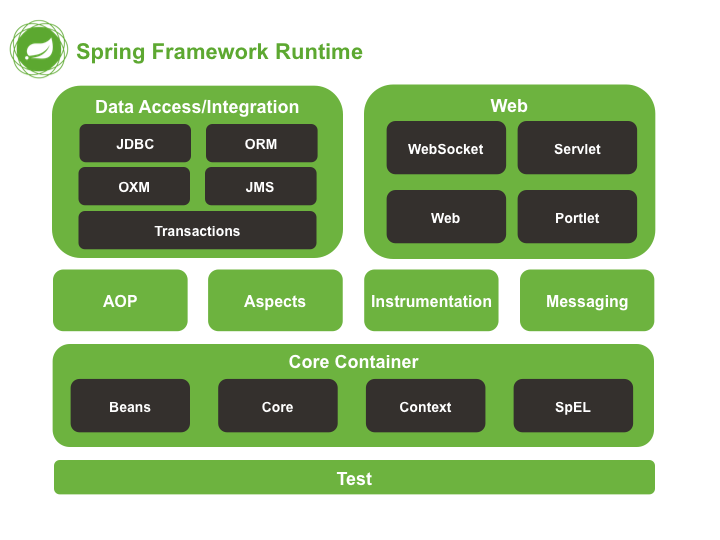
\includegraphics[width=15cm]{img/spring_runtime.png}
  \captionof{figure}{Spring Framework Runtime}
\end{center}

\subsubsection{Điểm mạnh của Framework Spring}

Dưới đây là danh sách các lợi ích tuyệt vời của việc sử dụng Spring Framework:
\begin{itemize}
    \item Spring cho phép các nhà phát triển tạo các ứng dụng cấp Enterprise sử dụng các POJO. Lợi ích của việc sử dụng các POJO là bạn không cần một sản phẩm chứa EJB như một máy chủ ứng dụng, mà bạn chỉ có thể sử dụng một bộ chứa servlet mạnh mẽ như Tomcat hoặc một số sản phẩm thương mại khác.
    \item Spring được tổ chức theo kiểu mô đun. Mặc dù số lượng các gói và các lớp là khá nhiều, nhưng bạn chỉ cần quan tâm đến những gì bạn cần và không cần quan tâm đến phần còn lại.
    \item Spring sử dụng một số công nghệ hiện có như một số ORM Framework, logging frameworks, JEE, Quartz, JDK timers và các công nghệ View khác.
    \item Dễ dàng để kiểm thử một chương trình được viết bằng Spring.
    \item Web framework của Spring là một Web MVC framework có thiết kế tốt, nó là một thay thế tuyệt vời cho Struts và các công nghệ kém phổ biến khác.
    \item Spring cung cấp một API thuận tiện để dịch các ngoại lệ công nghệ cụ thể (ném bởi JDBC, Hibernate, hoặc JDO chẳng hạn) vào các trường hợp ngoại lệ nhất quán, không được kiểm soát.
    \item IoC Container có trọng lượng nhẹ. Điều này có lợi cho việc phát triển và triển khai các ứng dụng trên các máy tính có bộ nhớ và tài nguyên CPU hạn chế.
    \item Spring cung cấp một giao diện quản lý transaction nhất quán có thể mở rộng đến một local transaction (ví dụ như sử dụng một cơ sở dữ liệu) và mở rộng lên các global transaction (sử dụng JTA).
\end{itemize}
\subsection{Python}
\subsubsection{Python là gì}

\begin{center}
  \captionsetup{type=figure}
  \includesvg[width=12cm]{img/python.svg}
  \captionof{figure}{Python}
\end{center}

Python là một ngôn ngữ thông dịch bậc cao, đa mục đích được tạo bởi Guido van Rossum vào năm 1991. Python được thiết kế với ưu điểm mạnh là dễ đọc, dễ học và dễ nhớ. Python là ngôn ngữ có hình thức rất sáng sủa, cấu trúc rõ ràng, thuận tiện cho người mới học lập trình. Cấu trúc của Python còn cho phép người sử dụng viết mã lệnh với số lần gõ phím tối thiểu.
\subsubsection{Đặc điểm của Python}
\begin{itemize}
    \item \textbf{Ngôn ngữ lập trình đơn giản, dễ học:} Python có cú pháp rất đơn giản, rõ ràng. Nó dễ đọc và viết hơn rất nhiều khi so sánh với những ngôn ngữ lập trình khác như C++, Java, C\#. Python làm cho việc lập trình trở nên thú vị, cho phép bạn tập trung vào những giải pháp chứ không phải cú pháp.
    \item \textbf{Miễn phí, mã nguồn mở:} Bạn có thể tự do sử dụng và phân phối Python, thậm chí là dùng cho mục đích thương mại. Vì là mã nguồn mở, bạn không những có thể sử dụng các phần mềm, chương trình được viết trong Python mà còn có thể thay đổi mã nguồn của nó. Python có một cộng đồng rộng lớn, không ngừng cải thiện nó mỗi lần cập nhật.
    \item \textbf{Khả năng di chuyển:} Các chương trình Python có thể di chuyển từ nền tảng này sang nền tảng khác và chạy nó mà không có bất kỳ thay đổi nào. Nó chạy liền mạch trên hầu hết tất cả các nền tảng như Windows, MacOS, Linux.
    \item \textbf{Khả năng mở rộng và có thể nhúng:} Giả sử một ứng dụng đòi hỏi sự phức tạp rất lớn, bạn có thể dễ dàng kết hợp các phần code bằng C, C++ và những ngôn ngữ khác (có thể gọi được từ C) vào code Python. Điều này sẽ cung cấp cho ứng dụng của bạn những tính năng tốt hơn cũng như khả năng scripting mà những ngôn ngữ lập trình khác khó có thể làm được.
    \item \textbf{Ngôn ngữ thông dịch cấp cao:} Không giống như C/C++, với Python, bạn không phải lo lắng những nhiệm vụ khó khăn như quản lý bộ nhớ, dọn dẹp những dữ liệu vô nghĩa,... Khi chạy code Python, nó sẽ tự động chuyển đổi code sang ngôn ngữ máy tính có thể hiểu. Bạn không cần lo lắng về bất kỳ hoạt động ở cấp thấp nào.
    \item \textbf{Thư viện tiêu chuẩn lớn để giải quyết những tác vụ phổ biến:} Python có một số lượng lớn thư viện tiêu chuẩn giúp cho công việc lập trình của bạn trở nên dễ thở hơn rất nhiều, đơn giản vì không phải tự viết tất cả code. Ví dụ: Bạn cần kết nối cơ sở dữ liệu MySQL trên Web server? Bạn có thể nhập thư viện MySQLdb và sử dụng nó. Những thư viện này được kiểm tra kỹ lưỡng và được sử dụng bởi hàng trăm người. Vì vậy, bạn có thể chắc chắn rằng nó sẽ không làm hỏng code hay ứng dụng của mình.
    \item \textbf{Hướng đối tượng:} Mọi thứ trong Python đều là hướng đối tượng. Lập trình hướng đối tượng (OOP) giúp giải quyết những vấn đề phức tạp một cách trực quan. Với OOP, bạn có thể phân chia những vấn đề phức tạp thành những tập nhỏ hơn bằng cách tạo ra các đối tượng.
\end{itemize}
\subsubsection{Python được dùng ở đâu?}
\begin{itemize}
    \item \textbf{Lập trình ứng dụng web:} Ta có thể tạo web app có khả năng mở rộng (scalable) được bằng cách sử dụng framework và CMS (Hệ thống quản trị nội dung) được tích hợp trong Python. Vài nền tảng phổ biến để tạo web app là:  Django, Flask, Pyramid, Plone, Django CMS. Các trang như Mozilla, Reddit, Instagram và PBS đều được viết bằng Python.
    \item \textbf{Khoa học và tính toán:} Có nhiều thư viện trong Python cho khoa học và tính toán số liệu, như SciPy và NumPy, được sử dụng cho những mục đích chung chung trong tính toán. Và, có những thư viện cụ thể như: EarthPy cho khoa học trái đất, AstroPy cho Thiên văn học,... Ngoài ra, Python còn được sử dụng nhiều trong machine learning, khai thác dữ liệu và deep learning.
    \item \textbf{Tạo nguyên mẫu phần mềm:} Python chậm hơn khi so sánh với các ngôn ngữ được biên dịch như C++ và Java. Nó có thể không phải là lựa chọn tốt nếu nguồn lực bị giới hạn và yêu cầu về hiệu quả là bắt buộc. Tuy nhiên, Python là ngôn ngữ tuyệt vời để tạo những nguyên mẫu (bản chạy thử - prototype). Ví dụ, bạn có thể sử dụng Pygame (thư viện viết game) để tạo nguyên mẫu game trước. Nếu thích nguyên mẫu đó có thể dùng C++ để viết game thực sự.
    \item \textbf{Ngôn ngữ tốt để dạy lập trình:} Python được nhiều công ty, trường học sử dụng để dạy lập trình cho trẻ em và những người mới lần đầu học lập trình. Bên cạnh những tính năng và khả năng tuyệt vời thì cú pháp đơn giản và dễ sử dụng của nó là lý do chính cho việc này.
\end{itemize}
\subsubsection{Thế mạnh của Python}
\begin{itemize}
  \item \textbf{Đơn giản:} Cú pháp đơn giản giúp cho người lập trình dễ dàng đọc và tìm hiểu.
  \item \textbf{Tốc độ:} Python có tốc độ xử lý nhanh hơn so với ngôn ngữ PHP.
  \item \textbf{Tương tác:} Chế độ tương tác cho phép người lập trình thử nghiệm tương tác sửa lỗi của các đoạn mã.
  \item \textbf{Chất lượng:} Thư viện có tiêu chuẩn cao, Python có khối cơ sở dữ liệu khá lớn nhằm cung cấp giao diện cho tất cả các CSDL thương mại lớn.
  \item \textbf{Thuận tiện:} Python được biên dịch và chạy trên tất cả các nền tảng lớn hiện nay.
  \item \textbf{Mở rộng:} Với tính năng này, Python cho phép người lập trình có thể thêm hoặc tùy chỉnh các công cụ nhằm tối đa hiệu quả có thể đạt được trong công việc.
\end{itemize}
\subsubsection{Framework Django}
\begin{center}
  \captionsetup{type=figure}
  
\includegraphics[width=12cm]{img/django.png}
  \captionof{figure}{Django}
\end{center}

Django là một web framework miễn phí mã nguồn mở được viết bằng Python. Django sử dụng mô hình Model-View-Control (MVC). Django được phát triển bởi Django Software Foundation(DSF) – một tổ chức phi lợi nhuận độc lập.

Mục tiêu chính của Django là đơn giản hóa việc tạo các website phức tạp có sử dụng cơ sở dữ liệu. Django tập trung vào tính năng “có thể tái sử dụng” và “có thể tự chạy” của các component, tính năng phát triển nhanh, không làm lại những gì đã làm. Một số website phổ biến được xây dựng từ Django là Pinterest, Instagram, Mozilla, và Bitbucket.

Django là một trong những framework phát triển web được yêu thích nhất cho việc phát triển các ứng dụng Python. Framework Django cho phép nguyên lý DRY (Don't Repeat Yourself) 

Không như các framework khácc, framework full-stack sử dụng miễn phí và mã nguồn mở của Python bao gồm một số lượng lớn các tính năng tích hợp thay vì cung cấp chúng dưới dạng các thư viện riêng lẻ. Django sử dụng ORM của nó để ánh xạ các đối tượng vào các bảng cơ sở dữ liệu. Điều này cho phép code hoạt động trên các cơ sở dữ liệu khác nhau cũng như giúp việc di chuyển từ cơ sở dữ liệu này sang cơ sở dữ liệu khác dễ dàng hơn. Mặc dù Django có hỗ trợ cho MySQL, PostgreSQL, SQLite và Oracle Database, nhưng nó vẫn có thể hỗ trợ các cơ sở dữ liệu khác thông qua trình điều khiển của bên thứ ba.

\textbf{Các điểm nổi bật chính:}
\begin{itemize}
    \item Học tập nhanh. Tương tự Python, Django cũng rất dễ học, không như Ruby on Rails.
    \item Tự động tạo SQL tables. Django sẽ thay bạn làm công việc này khi bạn đã xác định được cấu trúc.
    \item Tạo forms. Khi bạn đã tạo được Form class trong Django và linked đến model, form generator trong Django sẽ đảm nhận render form, xác minh và lưu trưc data.
    \item Admin Interface. Tương tự SQL table, khi bạn đã xác định được cấu trúc, Django sẽ tạo một admin interface cho phép bạn quản lý database (không khác gì PhpMyAdmin được build-in trong Django cả.)
    \item Django Shell. Python shell, ngay trong môi trường của Django project, chính là lợi thế mà Django shell mang lại. Tính năng này rất hữu hiệu khi debug (thường khó thực hiện trên PHP hơn).
\end{itemize}

\subsubsection{Framework Flask}
\begin{center}
  \captionsetup{type=figure}
  
\includegraphics[width=12cm]{img/flask.png}
  \captionof{figure}{Flask}
\end{center}

Flask là một web frameworks, nó thuộc loại micro-framework được xây dựng bằng ngôn ngữ lập trình Python. Flask cho phép bạn xây dựng các ứng dụng web từ đơn giản tới phức tạp. Nó có thể xây dựng các api nhỏ, ứng dụng web chẳng hạn như các trang web, blog, trang wiki hoặc một website dựa theo thời gian hay thậm chí là một trang web thương mại. Flask cung cấp cho bạn công cụ, các thư viện và các công nghệ hỗ trợ bạn làm những công việc trên.

Flask là một micro-framework. Điều này có nghĩa Flask là một môi trường độc lập, ít sử dụng các thư viện khác bên ngoài. Do vậy, Flask có ưu điểm là nhẹ, có rất ít lỗi do ít bị phụ thuộc cũng như dễ dàng phát hiện và xử lý các lỗi bảo mật.

\textbf{Tính năng của Framework Flask:}
\begin{itemize}
    \item Phát triển máy chủ.
    \item Phát triển trình gỡ lỗi.
    \item Hỗ trợ sẵn sàng để kiểm thử đơn vị.
    \item Jinja2 templates.
    \item RESTful request dispatch.
    \item Hỗ trợ bảo mật cookie.
    \item Full WSGI compliant.
    \item Tài liệu mở rộng.
    \item Dựa trên Unicode.
    \item Khả năng tương thích công cụ dựa trên ứng dụng Google.
    \item Nhiều tiện ích mở rộng cho các tính năng mong muốn.
    \item Tính modular và thiết kế gọn nhẹ.
    \item ORM-agnostic.
    \item Độ linh hoạt cao.
    \item Cung cấp xử lý HTTP request.
    \item API có độc đáo và mạch lạc.
    \item Dễ dàng triển khai.
\end{itemize}

\textbf{Điểm mạnh của Framework Flask:}
\begin{itemize}
  \item \textbf{Flask là một micro web framework:} Flask là một micro web framework được viết bằng Python, không yêu cầu tool hay thư viện cụ thể nào. “Micro” không có nghĩa là thiếu chức năng mà “micro” theo triết lý thiết kế là cung cấp một lõi chức năng “súc tích” nhất cho ứng dụng web nhưng người dùng có thể mở rộng bất cứ lúc nào. Flask luôn hỗ trợ các thành phần tiện ích mở rộng cho ứng dụng như tích hợp cơ sở dữ liệu, xác thực biểu mẫu, xử lý upload, các công nghệ xác thực, template, email, RESTful..., chỉ khác là khi nào bạn muốn thì bạn mới đưa vào thôi. Người dùng có thể tập trung xây dựng web application ngay từ đầu trong một khoảng thời gian rất ngắn và có thể phát triển quy mô của ứng dụng tùy theo yêu cầu.
  \item \textbf{Flask dễ cài đặt và triển khai:} Sau khi cài đặt Python, để cài đặt Flask chỉ cần bạn gõ lệnh: pip install Flask Bây giờ chúng ta thử tạo ứng dụng web với câu chào Hello World!. Thật đơn giản bạn sẽ tạo một folder với tên folder là tên ứng dụng, sau đó, tạo một tập tin .py và viết code. Flask tập trung vào sự tối giản, cho phép chúng ta xây dựng ứng dụng nhanh hơn.
  \item \textbf{Flask thật sự phù hợp cho việc xây dựng các web application có quy mô vừa và nhỏ, các API và web services:} 
  \begin{itemize}
    \item Xây dựng web application rất giống với việc viết các module Python chuẩn, cấu trúc gọn gàng và rõ ràng.
    \item Thay vì cung cấp hết tất cả mọi thứ, Flask cung cấp cho người dùng các thành phần cốt lõi thường được sử dụng nhất của khung ứng dụng web như URL routing, request and response object, template...
    \item Với Flask, việc chọn component nào cho ứng dụng là việc của chúng ta. Điều này thật tuyệt, vì mỗi web application có những đặc điểm và tính năng riêng, nó không phần phải chứa các component mà nó không dùng.
\end{itemize}
  \item \textbf{Flask giúp ta tập trung xây dựng ý tưởng, mục tiêu của riêng mình:} Flask có kiến trúc nhỏ, gọn nên bạn hoàn toàn không bị bó buộc bởi bộ khung cồng kềnh, không gặp bất cứ khó khăn nào khi cấu hình hay tổ chức ứng dụng. Không những thế, Flask còn có các ưu điểm nổi bật như: cực kỳ linh hoạt, tối giản, dễ tìm hiểu và sử dụng, định tuyến dễ dàng, rất dễ mở rộng. Vì vậy, công việc chính của ta là chỉ cần xác định ý tưởng, mục tiêu, tập trung vào việc xây dựng ứng dụng web mà thôi.
  \item \textbf{Nguồn tài liệu tham khảo về Flask rất phong phú:} Flask cung cấp rất nhiều tài liệu từ cài đặt đến thực hiện và triển khai, từ hướng dẫn nhanh đến hướng dẫn chi tiết. Ta có thể dễ dàng tìm kiếm, tham khảo, học tập về lập trình web application với Flask framework miễn phí trên Internet.
  \item \textbf{Cộng đồng Flask khá lớn:} Ta có thể dễ dàng, nhanh chóng tìm được giải pháp từ cộng đồng người sử dụng Flask mỗi khi gặp vấn đề cần giúp đỡ ví dụ như gặp lỗi, cách cài đặt thư viện, cách triển khai ứng dụng.
  \item \textbf{Mức độ phổ biến:} Có nhiều khách hàng đặt web application được xây dựng từ Flask Framework như Pinterest, LinkedIn, Twilio, Reddit, Netflix, Uber…
\end{itemize}
\subsection{NodeJS}
\subsubsection{NodeJS là gì}

\begin{center}
  \captionsetup{type=figure}
  \includesvg[width=10cm]{img/nodejs.svg}
  \captionof{figure}{NodeJS}
\end{center}


NodeJS là một mã nguồn được xây dựng dựa trên nền tảng Javascript V8 Engine, nó được sử dụng để xây dựng các ứng dụng web như các trang video clip, các forum và đặc biệt là trang mạng xã hội phạm vi hẹp. NodeJS là một mã nguồn mở được sử dụng rộng bởi hàng ngàn lập trình viên trên toàn thế giới. NodeJS có thể chạy trên nhiều nền tảng hệ điều hành khác nhau từ Windows cho tới Linux, OSX nên đó cũng là một lợi thế. NodeJS cung cấp các thư viện phong phú ở dạng Javascript module khác nhau giúp đơn giản hóa việc lập trình và giảm thời gian ở mức thấp nhất.

\subsubsection{Đặc điểm của NodeJS}

\begin{itemize}
  \item \textbf{Realtime:} Đây là tính năng quan trọng nhất của NodeJS. Realtime ở đây chính là xử lý giao tiếp từ client tới máy chủ theo thời gian thực. Giống như khi bạn lướt Facebook thì mỗi khi bạn comment hay like một topic nào đó thì ngay lập tức chủ topic và những người đã comment trên đó sẽ nhận được thông báo là bạn đã comment.
  \item \textbf{Không đồng bộ:} Tất cả các API của NodeJS đều không đồng bộ (none-blocking), nó chủ yếu dựa trên nền của NodeJS Server và chờ đợi Server trả dữ liệu về. Việc di chuyển máy chủ đến các API tiếp theo sau khi gọi và cơ chế thông báo các sự kiện của Node.js giúp máy chủ để có được một phản ứng từ các cuộc gọi API trước (Realtime).
  \item \textbf{Chạy rất nhanh:} NodeJ được xây dựng dựa vào nền tảng V8 Javascript Engine nên việc thực thi chương trình rất nhanh.
  \item \textbf{Đơn luồng nhưng khả năng mở rộng cao:} Node.js sử dụng một mô hình luồng duy nhất với sự kiện lặp. cơ chế tổ chức sự kiện giúp các máy chủ để đáp ứng một cách không ngăn chặn và làm cho máy chủ cao khả năng mở rộng như trái ngược với các máy chủ truyền thống mà tạo đề hạn chế để xử lý yêu cầu. Node.js sử dụng một chương trình đơn luồng và các chương trình tương tự có thể cung cấp dịch vụ cho một số lượng lớn hơn nhiều so với yêu cầu máy chủ truyền thống như Apache HTTP Server.
  \item \textbf{Không đệm:} NodeJS không đệm bất kì một dữ liệu nào và các ứng dụng này chủ yếu là đầu ra dữ liệu.
  \item \textbf{Có giấy phép:} NodeJS đã được cấp giấy phép bởi MIT License.
\end{itemize}

\subsubsection{NodeJs được sử dụng ở đâu}
\begin{itemize}
  \item \textbf{Websocket server:} Các máy chủ web socket như là Online Chat, Game Server…
  \item \textbf{Fast File Upload Client:} Là các chương trình upload file tốc độ cao.
  \item \textbf{Ad Server:} Các máy chủ quảng cáo.
  \item \textbf{Cloud Services:} Các dịch vụ đám mây.
  \item \textbf{RESTful API:} Đây là những ứng dụng mà được sử dụng cho các ứng dụng khác thông qua API.
  \item \textbf{Any Real-time Data Application:} Bất kỳ một ứng dụng nào có yêu cầu về tốc độ thời gian thực. Micro Services: Ý tưởng của micro services là chia nhỏ một ứng dụng lớn thành các dịch vụ nhỏ và kết nối chúng lại với nhau. Nodejs có thể làm tốt điều này.
\end{itemize}

\subsubsection{Thế mạnh của NodeJS}
\begin{itemize}
  \item Cú pháp ngắn gọn, dễ nhớ. Đặc biệt dễ học với những ai đã từng làm việc với nhiều với Javascript, Jquery.
  \item Xử lý không đồng bộ tốt: ví dụ khi upload file, chương trình không chờ việc upload xong mới xử lý việc tiếp theo. Nghĩa là trong khi xử lý upload file chương trình vẫn tiếp tục xử lý các công việc mới.
  \item Khả năng xử lý song song tuyệt vời: NodeJs sẽ tận dụng tối đa Unix để hoạt động. Tức là NodeJs có thể xử lý hàng nghìn process và trả ra 1 luồng khiến cho hiệu xuất hoạt động đạt mức tối đa nhất.
  \item Có nhiều packages hỗ trợ để tạo nhiều chức năng cho site, các packages được cài đặt bằng câu lệnh giống như cài đặt gem trong ruby on rails.
  \item Hỗ trợ nhiều template engine để render view.
  \item Có nhiều framework. Được sử dụng phổ biến nhất là : ExpressJs, SailsJS.
  \item Khả năng sử dụng lại code: dễ dàng tạo ra các module, helper, library để sử dụng ở nhiều nơi.
  \item Hỗ trợ security tốt. NodeJs mặc định hỗ trợ chống tấn công Cross-site script.
\end{itemize}

\subsubsection{ExpressJS}
\begin{center}
  \captionsetup{type=figure}
  
\includegraphics[width=15cm]{img/expressjs.png}
  \captionof{figure}{Express JS}
\end{center}

Express.js được xây dựng bởi TJ Holowaychuk, một thành viên trong team Node đã tạo ra Node.js. Cũng chính vì vậy mà đây là một trong những framework quan trọng nhất của Node.js. Expressjs cung cấp các hàm HTTP và midleware để tạo ra API đơn giản và dễ sử dụng. Express.js là một framework tối giản để xây dựng một loạt các ứng dụng web và di động cũng như các giao diện lập trình ứng dụng (API). Được ủng hộ bởi một cộng đồng lớn, framework này luôn được cập nhật liên tục và cải thiện tất cả những tính năng cốt lõi. Express.js cung cấp nhiều tính năng khác nhau như đơn giản hóa nhiều định tuyến, tích hợp cơ sở dữ liệu … và nhờ đó được dùng cho những ứng dụng phổ biến trên các trang web như MySpace, Geekli.st, Klout, Segment.io và Yummly.

ExpressJS được phát hành theo giấy phép mã nguồn mở, có cộng đồng hỗ trợ lớn, được phép sử dụng cho ứng dụng có mục đích thương mại.

Cấu trúc thư mục dự án khi sử dụng ExpressJS được chia là 3 phần: routes, Views và Public. ExpressJS xây dựng ứng dụng web theo đúng mô hình MVC (Model - View - Controller).

\textbf{Một số chức năng chính của ExpressJS:}
\begin{itemize}
  \item Hỗ trợ middleware để trả về các HTTP request.
  \item Định nghĩa route dựa trên các action của HTTP (CRUD).
  \item Cho phép trả về các trang html sử dụng các template engine (jade, pug…).
\end{itemize}

\subsubsection{Middleware trong ExpressJS:}

Middleware trong ngành công nghệ phần mềm được định nghĩa là một phần mềm có nhiệm vụ làm cầu nối (bridge), cung cấp các dịch vụ từ phía hệ điều hành đến các ứng dụng, giúp các ứng dụng có thể tương tác với các thành phần được hệ điều hành cho phép. Middleware được coi là chất kết dính dữa các phần mềm với nhau.

\textbf{Middleware trong Web:} 

Với tư tưởng chung là cầu nối giữa tương tác của người dùng và phần nhân của hệ thống, trong lập trình Web, Middleware sẽ đóng vai trò trung gian giữa request/response (tương tác với người dùng) và các xử lý logic bên trong web server.Do đó, Middleware trong các Framework lập tình Web (Django, Rails, ExpressJS), sẽ là các hàm được dùng để tiền xử lý, lọc các request trước khi đưa vào xử lý logic hoặc điều chỉnh các response trước khi gửi về cho người dùng.

\begin{center}
  \captionsetup{type=figure}
  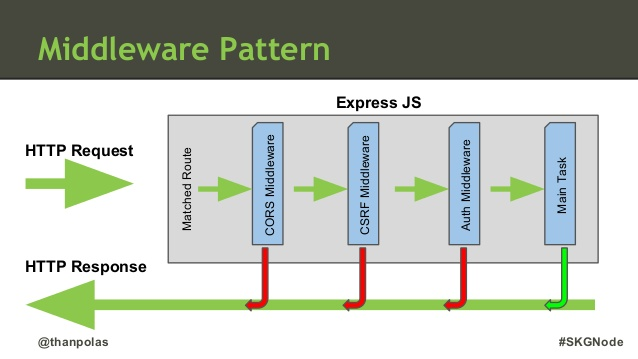
\includegraphics[width=15cm]{img/expressjsmiddleware.jpg}
  \captionof{figure}{Middleware trong ExpressJS}
\end{center}

Hình trên mô tả 3 middleware có trong ExpressJS. Một request khi gửi đến Express sẽ được xử lý qua 5 bước như sau :
\begin{itemize}
  \item Tìm Route tương ứng với request.
  \item Dùng CORS Middleware để kiểm tra cross-origin Resource sharing của request.
  \item Dùng CRSF Middleware để xác thực CSRF của request, chống fake request.
  \item Dùng Auth Middleware để xác thực request có được truy cập hay không.
  \item Xử lý công việc được yêu cầu bởi request (Main Task).
\end{itemize}

Bất kỳ bước nào trong các bước 2, 3, 4 nếu xảy ra lỗi sẽ trả về response thông báo cho người dùng, có thể là lỗi CORS, lỗi CSRF hay lỗi auth tùy thuộc vào request bị dừng ở bước nào.
\textbf{Middleware trong ExpressJS:} 

ExpressJS khi hoạt động, về cơ bản sẽ là một loạt các hàm Middleware được thực hiện liên tiếp nhau. Sau khi đã thiết lập, các request từ phía người dùng khi gửi lên ExpressJS sẽ thực hiện lần lượt qua các hàm Middleware cho đến khi trả về response cho người dùng. Các hàm này sẽ được quyền truy cập đến các đối tượng đại diện cho Request - req, Response - res, hàm Middleware tiếp theo - next, và đối tượng lỗi - err nếu cần thiết.

Một hàm Middleware sau khi hoạt động xong, nếu chưa phải là cuối cùng trong chuỗi các hàm cần thực hiện, sẽ cần gọi lệnh next() để chuyển sang hàm tiếp theo, bằng không xử lý sẽ bị treo tại hàm đó.

Các chức năng mà middleware có thể thực hiện trong ExpressJS sẽ bao gồm :
\begin{itemize}
  \item Thực hiện bất cứ đoạn code nào.
  \item Thay đổi các đối tượng request và response.
  \item Kết thúc một quá trình request-response.
  \item Gọi hàm middleware tiếp theo trong stack.
\end{itemize}

Trong Express, có 5 kiểu middleware có thể sử dụng :
\begin{itemize}
  \item Application-level middleware (middleware cấp ứng dụng).
  \item Router-level middleware (middlware cấp điều hướng - router).
  \item Error-handling middleware (middleware xử lý lỗi).
  \item Built-in middleware (middleware sẵn có).
  \item Third-party middleware (middleware của bên thứ ba).
\end{itemize}
\subsection{Sự lựa chọn}
Chúng ta có thể thấy Java là một ngôn ngữ mạnh, linh hoạt, bảo mật cao, viết một lần thực thi khắp nơi. Tuy nhiên vì Java chạy trên máy ảo Java Virtual machine, đây vừa là điểm mạnh khi Java có thể chỉ cần viết một lần thực thi khắp nơi, tuy nhiên nó cũng khiến Java chậm đi rất nhiều và tiêu thụ nhiều bộ nhớ, khiến cho ứng dụng ngày càng nặng nề khi xử lý nhiều kết nối.

Python là một ngôn ngữ rất dễ học, dễ sử dụng, có cú pháp đơn giản, cộng đồng hỗ trợ lớn, nhiều công cụ và công nghệ hỗ trợ. Đây cũng là ngôn ngữ mà được rất nhiều người yêu thích, tuy nhiên Python lại có những hạn chế như tốc độ khá chậm, chạy đơn luồng, vì vậy sẽ không thể đáp ứng được khi ứng dụng càng ngày càng có nhiều kết nối.

NodeJS có đặc điểm là tốc độ rất nhanh, xử lý nhiều kết nối tốt, dễ dàng mở rộng để phát triển, thích hợp. Đây là những đặc tính đặc biệt thích hợp cho hệ thống Tổ chức hành chính với những đặc thù công việc như hay thay đổi nghiệp vụ, xuất báo cáo định kỳ, theo yêu cầu, truy cập lượng lớn hồ sơ nhân viên. Vì vậy nhóm quyết định sử dụng NodeJS cùng với công nghệ ExpressJS cho phía server của hệ thống này.